\section{Durchführung}
\label{sec:Durchführung}

\begin{figure} [H]!
    \centering
    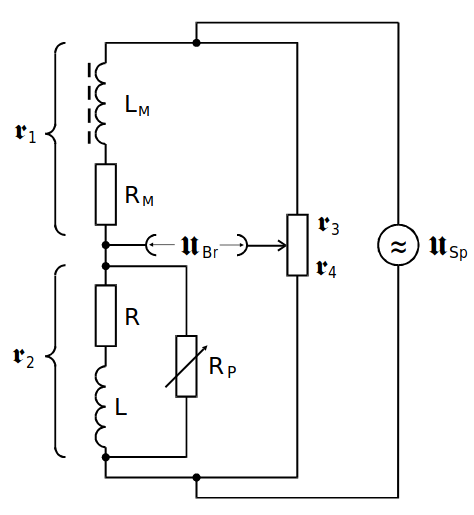
\includegraphics[scale=0.5]{content/bild1.png}
    \caption{Brückenschaltung zur Suszeptibilitätsmessung [1]}
    \label{fig:plot1}
  \end{figure}

Zur Messung der Suszeptibilität wird die Brückenschaltung
gemäß Abbildung \ref{fig:plot1} verwendet. Die durch diese Schaltung
aufkommenden Störspannungen werden durch einen Frequenzfilter,
einen Bandpass herausgefiltert und die gesuchte
Brückenspannung verstärkt.

Zunächst gilt es,
die Durchlassfrequenz des Filters durch Messung der
Ausgangsspannung mit einem Mikrovoltmeter zu bestimmen.
Gemessen wird die Ausgangsspannung $U_A$ in dreißig Schritten
für Frequenzen zwischen Frequenzen von $\nu = \SI{20}{\kilo\hertz}$ und
$\SI{40}{\kilo\hertz}$. Dabei sollten Schritte zwischen den Messungen
nahe des Maximums kleingehalten werden.

\begin{figure} [H]!
    \centering
    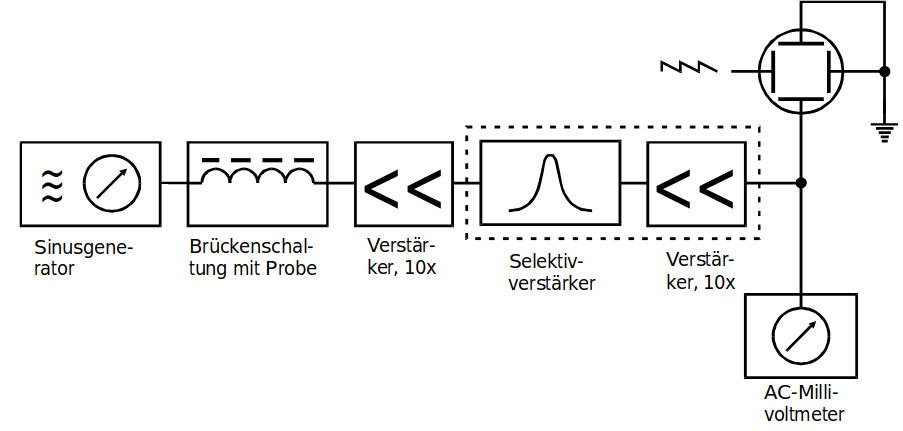
\includegraphics[scale=0.3]{content/bild2.png}
    \caption{Blockschaltbild des Versuchsaufbaus [1]}
    \label{fig:plot2}
  \end{figure}

Zur eigentlichen Messung wird der Aufbau, der on Abbildung \ref{fig:plot2}
dargestellt ist, verwendet. Zunächst wird die Frequenz der eingehenden Sinusspannung
auf den Wert der Durchlassfrequenz des Bandpasses geregelt. Danach werden die
Brückenspannung $U_\text{B}$ mithilfe der Abgleichwiderstände $R_3 / R_4$ und $R_\text{P}$
abgeglichen und die Werte von $R_3 / R_4$ und $U_\text{B}$ notiert. Für letztere wird der
Wert nochmals nach Einführung der Stoffprobe in die Spule notiert.
Für die alternative Methode mit der Gleichung /eqref{eqn:alternativ} 
muss die Brückenspannung nochmals nach Einführung der Probe abgeglichen und ihr Wert,
sowie der von $R_3 / R_4$ notiert werden.
Für die Proben $\symup{Dy_2O_3}$, $\symup{C_6O_{12}Pr_3}$, 
$\symup{Gd_2O_3}$ und $\symup{Nd_2O_3}$ werden jeweils drei Messungen durchgeführt.
Zuletzt werden noch die jeweiligen Längen und Massen der Proben bestimmt.





